\chapter{Généralités sur les méthodes Agiles}
	\nouveauChapitre
	\section{Historique}
		En 1968 à eu lieu la naissance du Génie Logiciel, nous sommes passé de la programmation non structurelle à la programmation structurelle avec Cobol et Fortran
		Cela à permis d'avancer, avec de nouveaux langages, des OS principalement mais aussi avec :

		Les premières méthodes méthodes remontent à 1994 avec Scrum et 1996 avec l'Extreme Programming, de nos jours, les deux disciplines ont tendances à se rapprocher.
		\begin{itemize}
			\item Le cycle en V (Aproche séquentielle)
			\item L'hyper-management (Taylorisme)
			\item L'hyper-formalisme (exigences, conception)
			\item L'obsession de la mesure et métrique
		\end{itemize}
		\paragraph{} Le terme ``Agile'' apparaît en 2001 (Snowbird, rédaction du ``manifest''), il est apparut pour répondre aux malaises énoncés en Avant-propos page \pageref{avantPropos}.


		Dans les méthodes Agile on essaye de mettre l'humain et le relationnel au centre du développement. Par exemple les problèmes doivent être résolus en face à face.
		Le \textbf{client} est au centre du développement, on part de l'idée que le client va changer d'idée, et donc qu'on le contacter régulièrement pour 
		connaître son avis, et ses éventuels changements.

		Elles ont également un ensemble de règles, que l'équipe se doit de respecter.
		\exemple{Extreme Programming
			\begin{itemize}
				\item Le code au centre de tout
				\item Programmation en binome (Importance de la qualité)
				\item Tests unitaires
				\item Meeting réguliers (tous les jours)
				\item Tests de validation
				\item Iterations
			\end{itemize}
			}
%	\section*{\bsc{TDD}}
%	\begin{enumerate}
%		\item Test
%		\item Code
%		\item Refactoring
%	\end{enumerate}
%	Cette méthode demande à ce que que les tests soient rédigés avant le développement, une fois les tests rédigés, il faut créer un programme avec lequel tous les tests passent. Cela necessite donc de bien 
%	comprendre le problème dès le départ, et de savoir ce que nous souhaitons obtenir.
\newpage
	\section{Caractéristiques des méthodes Agiles}
		Il existe une multitude de méthode Agiles différentes, cependant, elles ont toutes les même caractéristiques et le même but d'avoir un projet aboutit qui aura couté le moins cher possible.
		\subsection{L'humain est au centre du développement} \label{client}
		En effet, dans les méthodes Agiles, l'Humain est le plus important, autrement dit,\textbf{ le client} doit être vu très régulièrement, pour qu'il puisse donner son avis sur le projet, et éventuelleemnt
		donner l'avancée de sa réflexion sur ses besoins.

		Également, l'\textbf{équipe} doit être soudée, et investit dans son projet, elle doit participer d'un bout à l'autre du projet, il est ainsi indispensable d'avoir des équipes petites afin d'éviter aux développeurs
		de se sentir noyés dans la masse.
		\subsection{La qualité au centre du développement}
		Avoir un travail de qualité induit donc que le programme final devra correspondre au client comme expliqué en section \ref{client}, mais également ne doit pas être bugué, ainsi
		les \textbf{tests} sont extrêmements important.

		Le programme devra lui aussi avoir été codé avec le plus grand soins, afin d'avoir un \textbf{code propre} qui permettra une maintenance facile, pour cela certaines méthode Agiles préconisent la programmation en binôme.
		\subsection{Méthodes Agiles Versus Méthodes classiqus}
		\begin{figure}[H]
			\center
			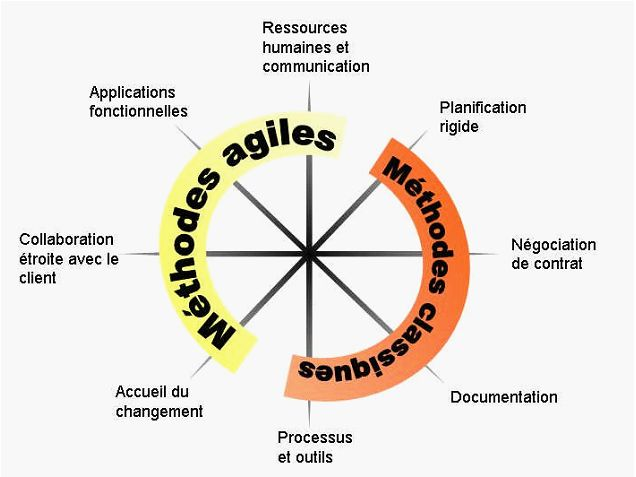
\includegraphics[width=10cm]{images/1-caracAgiles.jpg}
			\caption{Caractéristiques des méthodes Agiles}
		\end{figure}
		
%		\begin{itemize}
%			\item Adaptatives plutôt que prédictives
%			\item Orientées vers les personnes plutôt que vers les processus
%			\item Impose au chef de projet de conserver à l'esprit que l'objectif est une aplication et non un modèle
%		\end{itemize}
%		Ces 4 valeurs peuvent induire des principes généraux. 
%		\begin{itemize}
%			\item La priorité est de satisfaire le client en lui livrant très tôt des versions
%			\item Accueillir le changement à bras ouverts, même tard dans le processus de développement
%			\item Livrer le plus souvent possible des versions opérationneles de l'application avec une fréquence compris entre 2 semaines et 3 mois
%			\item Clients et développeuers doivent coopérer quotidiennement tout au long du projet
%			\item Construire des projets autour d'individus motivés
%			\item La méthode la plus efficace pour communiquer des informations reste la communication en face à face
%			\item Le fonctionnement de l'application est le premier indicateur d'avancement du projet
%			\item Les méthodes agiles recommandent que le projet avance à un rythme soutenable
%			\item Porter une attention continue à l'excellence technique et la conception améliore l'agilité
%			\item La simplicité est essentielle
%			\item Les meilleurs architecutres, spécifications et conceptions sont le fruit d'équipes qui s'auto organisent
%			\item À intervalles de temps réguliers, l'ensemble de l'équipe s'interroge sur la manière de devenir encore plus effiace
%		\end{itemize}
		
	\section{Panorama de différentes méthode sagiles}
	Nous allons étudier très rapidement les différentes méthodes Agiles qui peuvent exister, ce sont les méthodes Agiles les plus utilisées: 
	\begin{itemize}
		\item UP
		\item eXtreme Programming
		\item Dynamic Software Development Method
		\item Adaptive Software Development
		\item Crystal Clear
		\item \bsc{scrum}
	\end{itemize}
	\subsection{UP}
		Les fondamentaux d'UP: 
		\begin{itemize}
			\item Pilotage par les cas d'utilisation
			\item Centré sur l'architecture
			\item Itérative et incrémentale
			\item Gère les besoins et les exigences
			\item Fondée sur la production de de composants 
			\item Pratique la modélisation visuelle
			\item Surveille la qualité et les risques
		\end{itemize}
		\vspace{3cm}
		\begin{figure}[H]
			\center
			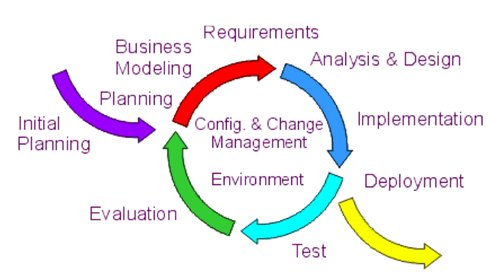
\includegraphics[width=10cm]{images/2-up.jpg}
			\caption{Cycle de vie de UP}
		\end{figure}
		\begin{figure}[H]
			\center
			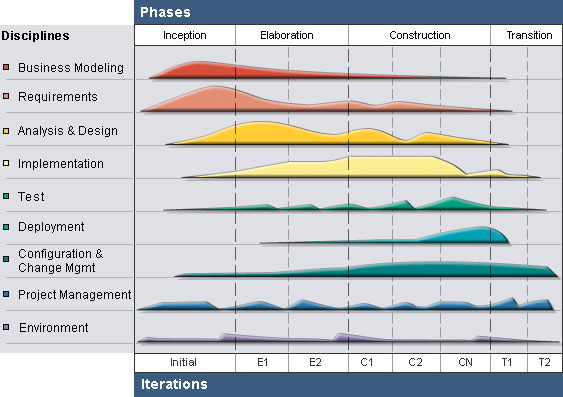
\includegraphics[width=14cm]{images/3-up.jpg}
			\caption{Phases de développement de UP}
		\end{figure}
	\subsection{eXtreme Programming}
	Les créateurs sont Ward \bsc{Cunningham} et Kent \bsc{Beck}. 
	\subsubsection{Valeurs clefs}
	\paragraph{Communication} Rendre la communication omniprésente entre tous les intervenants
	\paragraph{Simplicité} Il coûte moins cher d'aller au plus simple et de rajouter des fonctionnalités par la suite plutôt que de concevoir dès le départ un
	système très compliqué dont on risque de n'avoir jamais l'utilité
	\paragraph{Feedback} Indispensable pour que le projet puisse accueillir le changement
	\paragraph{Courage} Concerne aussi bien les développeurs que le client
	\subsubsection{Quelques pratiques}	
		\begin{itemize}
			\item Planning game
			\item Petites releases
			\item Métaphores pour décrire l'architecture
			\item COnception simple
			\item Tests
			\item Refactoring 
			\item Programmation en binôme
			\item Propriété collective
			\item Intégration continue
			\item Pas de surcharge de travail
			\item Client sur site
			\item Standars de code (conventions)
		\end{itemize}
		\begin{figure}[H]
			\center
			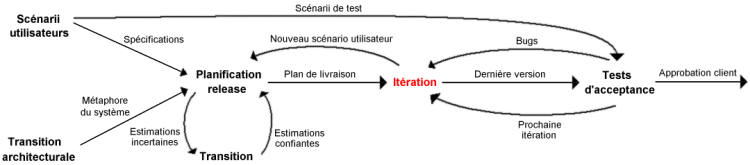
\includegraphics[width=12cm]{images/4-extremeProgramming.png}
			\caption{Cycle de vie de eXtreme Programming}
		\end{figure}
		
	\subsection{Dynamic Software Development Method}
	DSDM\footnote{Dynamic Software Development Method} possèdent à peu près les même principes que les autres méthodes. Elle trouve ses origines en Angleterre au début des années 1990. 
	L'idée fondamentale derrière cette méthode est de fixer le temps et les ressources et de faire varier le nombre de fonctionnalités en conséquence.
	\begin{itemize}
		\item Implication actives des utilisateurs
		\item Equipes autorisées à prendre des décisions
		\item Produit rendu tangible aussi souvent que possible
		\item L'adéquiation au besoin métier est le critère essentiel pour l'acceptation des fournitures
		\item UN dévelopement itératif et incrémental permet de converger vers une solution appropriée
		\item Toute modification pendant la réalisation est réversible
		\item Besoins définis à un niveau de synthèse
		\item Tests intégrés pendant tout le cycle de vie
		\item Esprit de coopération entre tous
	\end{itemize}
		\begin{figure}[H]
			\center
			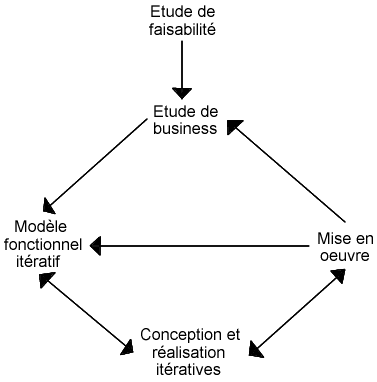
\includegraphics[width=6cm]{images/5-dsdm.png}
			\caption{Cycle de vie de DSDM}
		\end{figure}

	\subsection{Adaptive Software Development}
	La méthode ASD\footnote{Adaptive Software Development} à été crée par Jim \bsc{Highsmith}, elle possède 6 caractéristiques principales:
	\begin{itemize}
		\item Mission focused
		\item Component-based
		\item Iterate
		\item Timeboing
		\item Projet risk-driver
		\item Responding to change
	\end{itemize}
	\subsubsection{Spéculer}
	\begin{itemize}
		\item Initier le projet
		\item Déterminer la date butoir du projet
		\item Définir le nombre d'itérations et les dates associées
		\item Donner une missions à chaque itération
		\item Affecter les composants de base aux itérations
		\item Affecter les technologies aux itérations
		\item Développer une liste de tâche à réaliser
	\end{itemize}
	\subsubsection{Collaborer}
	\begin{itemize}
		\item Délivrance des composants
		\item Communication forte et assez informelle
		\item Possibilité d'apliquer des pratiques Agiles (de type XP)
	\end{itemize}
	\subsubsection{Apprendre}
	\begin{itemize}
		\item Contrôle qualité utilisateur / client
		\item COntrôle qualité technique
		\item Suivi de la performance
		\item Bilan sur l'état d'avancement
		\item COmmunication forte et assez informelle
		\item Possibilité d'appliquer des pratiques Agiles (de type XP)
	\end{itemize}
	% TODO
	\subsection{Crystal Clear}
	Méthode créée par Alistair \bsc{Cockburn}.
	\paragraph{Les points clefs}
	\begin{itemize}
		\item Importance de la communication et du feed-back client
		\item Releases fréquentes
		\item Deux grandes phases
			\begin{itemize}
				\item Conception et planning
				\item Itérations
			\end{itemize}
		\item Adapté à des équipes de 6 personnes maximum (pas de leadership clairement exprimé)
	\end{itemize}
	\subsection{\bsc{SCRUM}}
	La méthode scrum est expliqué en détaille au chapitre \ref{scrum} page \pageref{scrum}. 
	\section{Synthèse}
		%%% Graphique
		Les méthodes agiles semble adaptés à un besoin : 
		\begin{itemize}
			\item Pas de sous-traitance
			\item Équipe motivée
			\item Équipe légère
			\item Équipe peut nombreuse
			\item Environnement non critique
			\item Projet non complexe
		\end{itemize}
		\subsection{Comparaisons entre les méthodes}
			\begin{center}
				\begin{tabular}{|p{3.5cm}||p{7cm}|p{7cm}|}
					\hline
					\textbf{Méthodes} & \textbf{Dites classiques ou ``lourdes''} & \textbf{Dites nouvelles ou ``Agiles''}\\
					\hline
					Paradigme & Prédictivité & Adaptabilité \\
					\hline
					Fondement & Analytique cartésien & Pragmatique empiriste \\
					\hline
					Cycle projet & EN cascade & Incrémental et itératif \\
					\hline
					Risque & Descriptive &Expérimentation \\
					\hline
					Raisonnement & Discursifs & Systémique \\
					\hline
					Pensée & Réductionniste & Vision holistique \\
					\hline
					Philosophie d'analyse & Considère la nature des intéractions & Considère les effets des intéractions \\
					\hline
					Axe de recherche & L'analyse de la structure & L'aboutissement des actions \\
					\hline
					Conduit à des systèmes & À forte entropie & À forte rétroactivité \\
					\hline
					Philosophie d'action & Conduit à une action totalement détaillée et programmée & Conduit à une action par objectifs et flexible\\
					\hline
					Aboutit concrètement & À la reconduction de la structure existante & À l'amélioration des éléments de performance\\
					\hline
					Validation & Comparaison théorique à base de jeu d'essais en fin de parcours & Confrontation permanente du modèle avec la réalité (prototype)\\
					\hline
				\end{tabular}
			\end{center}

